\documentclass[handout]{beamer}
\usetheme{metropolis}

% -------------------------------------------------------------------
%   PAQUETES
% -------------------------------------------------------------------
\usepackage[spanish,activeacute]{babel}     % Soporte para español
\usepackage{amsmath, amssymb}              % Matemáticas esenciales
\usepackage{graphicx}                      % Inclusión de imágenes
\usepackage{multirow}                      % Tablas complejas
\usepackage[ruled,vlined,lined]{algorithm2e}% Algoritmos
\usepackage{fontspec}                      % Manejo de fuentes con XeLaTeX (REQUIRES XeLaTeX or LuaLaTeX engine)
\setsansfont{Lato}                         % Fuente Sans (make sure Lato is installed)
\setmonofont{Inconsolata}                  % Fuente Monospace (make sure Inconsolata is installed)
\usepackage{hyperref}                      % Enlaces clicables
\hypersetup{
    colorlinks=true,
    linkcolor=blue, % Consider using metropolis default colors? e.g., linkcolor=ocre
    urlcolor=magenta % Consider using metropolis default colors?
}
\usepackage{dsfont}                        % Símbolos matemáticos adicionales (\mathds{})
\usepackage{cases}                         % Entornos para casos matemáticos
\usepackage{epic}                          % Dibujos adicionales (Consider TikZ for more complex drawings)
\usepackage{framed,color}                  % Marcos y colores (Beamer provides similar environments)

% -------------------------------------------------------------------
%   CUSTOM COMMANDS (Added)
% -------------------------------------------------------------------
\newcommand{\vect}[1]{\mathbf{#1}} % Define \vect for bold vectors
\newcommand{\mat}[1]{\mathbf{#1}}  % Define \mat for bold matrices

% -------------------------------------------------------------------
%   INFORMACIÓN DEL DOCUMENTO
% -------------------------------------------------------------------
\title{Procesamiento del Lenguaje Natural}
\subtitle{Redes Neuronales Recurrentes (RNN)}
\author[Jorge Ortiz Fuentes]{Jorge Ortiz Fuentes}
\date{\today}

% -------------------------------------------------------------------
%   METADATOS / CONFIGURACIONES
% -------------------------------------------------------------------
\setbeamercolor{normal text}{fg=black,bg=white} % Overrides theme defaults, ensure this is intended
\setbeamercolor{alerted text}{fg=red!80!black}
\setbeamercolor{example text}{fg=green!50!black}
\setbeamertemplate{navigation symbols}{} % Hides navigation buttons
\setbeamertemplate{caption}[numbered]     % Numbers figure/table captions
\setbeamertemplate{footline}{             % Custom footline
  \begin{beamercolorbox}[wd=\paperwidth,ht=2.5ex,dp=1ex]{frametitle} % Use frametitle color scheme
    \vspace{1pt} % Minimal space from top of box
    \hfill\insertframenumber/\inserttotalframenumber\hspace{3mm} % Page number right-aligned
  \end{beamercolorbox}
}
\metroset{block=fill} % Use filled blocks (standard for Metropolis)

% -------------------------------------------------------------------

\begin{document}

% --- PORTADA ---
\begin{frame}[plain]
  \titlepage
\end{frame}

% --- ÍNDICE ---
\begin{frame}{Contenido}
  \tableofcontents
\end{frame}

% ===================================================================
\section{Introducción y motivación}
% ===================================================================

\begin{frame}
    \frametitle{Consideraciones sobre el lenguaje}
    \begin{block}{El lenguaje es secuencial}
        \begin{itemize}
            \item El lenguaje natural (texto, habla) es inherentemente \textbf{secuencial} y el significado de las palabras depende de su \textbf{contexto}.
            \item Los modelos \textit{feed-forward} tradicionales procesan entradas de forma independiente, carecen de ``memoria''. % Corrected quote
        \end{itemize}
    \end{block}
    \begin{alertblock}{Necesidad de memoria}
        Requerimos modelos capaces de:
        \begin{itemize}
            \item Procesar secuencias de longitud variable.
            \item Mantener información de pasos anteriores (\textbf{memoria temporal}).
            \item Capturar dependencias entre elementos en la secuencia.
        \end{itemize}
    \end{alertblock}
\end{frame}

% ===================================================================
\section{Redes Neuronales Recurrentes (RNN)}
% ===================================================================

\begin{frame}
    \frametitle{Abstracción de una RNN}
    \begin{columns}[T]
        \begin{column}{0.65\textwidth}
            \begin{block}{Idea central: recurrencia}
                \begin{itemize}
                    \item Una RNN procesa la secuencia paso a paso ($t=1, 2, ..., T$).
                    \item Mantiene un \textbf{estado oculto} ($\vect{h}_t$) que actúa como \textbf{memoria}.
                    \item En cada paso $t$:
                        \begin{itemize}
                            \item Recibe entrada $\vect{x}_t$.
                            \item Recibe estado anterior $\vect{h}_{t-1}$.
                            \item Calcula nuevo estado $\vect{h}_t$.
                            \item (Opcional) Produce salida $\vect{y}_t$.
                        \end{itemize}
                    \item El estado $\vect{h}_t$ resume la información relevante de $\vect{x}_1, ..., \vect{x}_t$.
                \end{itemize}
            \end{block}
        \end{column}
        \begin{column}{0.35\textwidth} % Adjusted column width slightly
            \begin{figure}
                \centering
                \includegraphics[width=0.7\textwidth]{pics/rnn_cell_loop.png} % Use \textwidth in column
                \vspace{1cm}
                \caption{Celda RNN básica.} % Shortened caption
            \end{figure}
        \end{column}
    \end{columns}
\end{frame}

\begin{frame}
    \frametitle{Desenrollada en el tiempo}
    \begin{block}{Recurrencia}
        El bucle recurrente puede ``desenrollarse'' en el tiempo, revelando una cadena de procesamiento.
    \end{block}
    \begin{figure}
        \centering
        \includegraphics[width=0.9\textwidth]{pics/rnn_unrolled.png}
         \vspace{1cm}
        \caption{RNN desenrollada para una secuencia de longitud T. }
    \end{figure}
\end{frame}

\begin{frame}
    \frametitle{Parámetros compartidos}
    \begin{alertblock}{Importancia}
        \textbf{Crucial:} los mismos parámetros se usan en \textbf{cada paso temporal}.
        \begin{itemize}
            \item Reduce drásticamente el número de parámetros a aprender.
            \item Permite generalizar a secuencias de diferente longitud.
            \item El modelo aprende una transición \textit{general} aplicable en cualquier punto de la secuencia.            
        \end{itemize}
    \end{alertblock}
\end{frame}

\begin{frame}
    \frametitle{RNN simple (Elman Network)}
        \begin{block}{Arquitectura básica (Elman, 1990)}
            \begin{itemize}
                \item Capa de entrada $\vect{x}_t$.
                \item Capa oculta recurrente $\vect{h}_t$.
                \item Capa de salida $\vect{y}_t$.
            \end{itemize}
        \end{block}
        \begin{block}{Ecuaciones (Conceptuales)} % Shortened title
            \begin{align*}
                \vect{h}_t &= f(\mat{W}_{xh} \vect{x}_t + \mat{W}_{hh} \vect{h}_{t-1} + \vect{b}_h) \\
                \vect{y}_t &= g(\mat{W}_{hy} \vect{h}_t + \vect{b}_y)
            \end{align*}
            \footnotesize Donde $f, g$ son activaciones, $\mat{W}$ pesos, $\vect{b}$ sesgos. % Shortened explanation
        \end{block}
\end{frame}


\begin{frame}
  \frametitle{Otra notación de las ecuaciones}
      \begin{block}{Formulas}
          \begin{align*}
              \vect{h}_t &= f(\mat{W} \vect{x}_t + \mat{U} \vect{h}_{t-1} + \vect{b_h}) \\
              \vect{y}_t &= g(\mat{V} \vect{h}_t + \vect{b_y})
          \end{align*}
  
          \begin{itemize}
              \item $\mat{W}$: matriz de pesos de \textbf{entrada actual} ($\vect{x}_t \rightarrow \vect{h}_t$)
              \item $\mat{U}$: matriz de pesos \textbf{recurrentes} ($\vect{h}_{t-1} \rightarrow \vect{h}_t$)
              \item $\mat{V}$: matriz de pesos de \textbf{salida} ($\vect{h}_t \rightarrow \vect{y}_t$)
              \item $f$: activación recurrente (típicamente $\tanh$ o $\text{ReLU}$)
              \item $g$: activación de salida (depende de la tarea)
          \end{itemize}
      \end{block}
\end{frame}

\begin{frame}
    \frametitle{Características de las RNN}
    \begin{block}{Ventajas}
        \begin{itemize}
            \item Conceptualmente simple.
            \item Capaz de procesar secuencias de longitud variable.
            \item Puede modelar dependencias temporales (en teoría).
            \item Menos parámetros que arquitecturas más complejas.
        \end{itemize}
    \end{block}
\end{frame}

\begin{frame}
    \frametitle{Características de las RNN}
    \begin{alertblock}{Limitaciones}
        \begin{itemize}
            \item \textbf{Problema del Gradiente Desvaneciente/Explosivo}: Dificultad para aprender dependencias a largo plazo. Gradientes se multiplican $\rightarrow$ muy pequeños (vanishing) o muy grandes (exploding).
            \item La memoria es ``frágil'': la información de pasos lejanos tiende a perderse o diluirse.
            \item Menos potente que arquitecturas más modernas (LSTM, GRU) para tareas complejas.
        \end{itemize}
    \end{alertblock}
    \begin{center} \bigskip
        \textit{Motivación para arquitecturas más sofisticadas.} % Shortened text
    \end{center}
\end{frame}


\begin{frame}
    \frametitle{Problema: gradientes desvanecientes / explosivos}
    \begin{columns}[T] % Keep T align here as blocks are distinct
        \begin{column}{0.5\textwidth}
            \begin{alertblock}{Gradiente Desvaneciente (Vanishing)}
                \begin{itemize}
                    \item<+-> Gradiente se reduce exponencialmente hacia atrás.
                    \item<+-> Multiplicación repetida de valores $< 1$.
                    \item<+-> \textbf{Consecuencia:} No aprende dependencias largas.
                \end{itemize}
                 
            \end{alertblock}
        \end{column}
        \begin{column}{0.5\textwidth}
            \begin{alertblock}{Gradiente Explosivo (Exploding)}
                \begin{itemize}
                    \item<+-> Gradiente crece exponencialmente hacia atrás.
                    \item<+-> Multiplicación repetida de valores $> 1$.
                    \item<+-> \textbf{Consecuencia:} Entrenamiento inestable (NaNs).
                \end{itemize}
                 
            \end{alertblock}
        \end{column}
    \end{columns}
    \begin{center} \visible<3->{\bigskip \textit{Principal obstáculo para las RNN simples.}} % Make text appear last
    \end{center}
\end{frame}

\begin{frame}
    \frametitle{Técnicas de mitigación}
    \begin{block}{Estrategias comunes}
        \begin{itemize}
            \item \textbf{Inicialización de pesos cuidadosa:} Evitar empezar en regiones de saturación o magnitudes extremas (ej. Xavier, He, Ortogonal).
            \item \textbf{Funciones de activación alternativas:} ReLU y variantes (ej. Leaky ReLU) pueden mitigar el desvanecimiento.
            \item \textbf{Arquitecturas con Compuertas (LSTM, GRU):} La solución más robusta, controlan el flujo de información/gradientes. \textbf{(Veremos a continuación)}
        \end{itemize}
    \end{block}
\end{frame}

% ===================================================================
\section{Variantes de RNN}
% ===================================================================

\begin{frame}
    \frametitle{RNN Bidireccionales (BiRNN): Motivación}
     \begin{block}{Motivación}
        En muchas tareas (ej. etiquetado, traducción), el contexto \textbf{futuro} es tan importante como el \textbf{pasado}.
        \begin{itemize}
            \item Ejemplo: Determinar si ``banco'' es \textit{institución financiera} o \textit{asiento} puede requerir ver palabras posteriores.
            \item Una RNN estándar solo ve el pasado ($\vect{h}_t$ depende de $t-1, t-2, ...$).
        \end{itemize}
    \end{block}
\end{frame}

\begin{frame}
    \frametitle{BiRNN: Arquitectura}
     \begin{columns}[T]
        \begin{column}{0.47\textwidth}
             \begin{block}{Arquitectura}
                \begin{itemize}
                    \item Dos RNNs independientes:
                        \begin{itemize}
                            \item Una \textbf{hacia adelante} ($\rightarrow$): captura $\overrightarrow{\vect{h}_t}$.
                            \item Una \textbf{hacia atrás} ($\leftarrow$): captura $\overleftarrow{\vect{h}_t}$.
                        \end{itemize}
                    \item Estados ocultos se \textbf{combinan} (ej. concatenan):
                    \[ \vect{h}_t = [\overrightarrow{\vect{h}_t}; \overleftarrow{\vect{h}_t}] \]
                    \item La salida $\vect{y}_t$ se basa en $\vect{h}_t$.
                \end{itemize}
            \end{block}
        \end{column}
        \begin{column}{0.53\textwidth}
             \begin{figure}
                \centering
                
                \includegraphics[width=\textwidth]{pics/birnn_concat.png}
                 \vspace{1cm}
                \caption{Arquitectura BiRNN. }
            \end{figure}
        \end{column}
    \end{columns}
\end{frame}

\begin{frame}
    \frametitle{BiRNN: Ventajas y Aplicaciones}
    \begin{block}{Ventajas}
        \begin{itemize}
            \item Acceso a contexto completo (pasado y futuro) en cada punto.
            \item Generalmente mejora el rendimiento en tareas donde el contexto global es útil.
        \end{itemize}
    \end{block}
\end{frame}

\begin{frame}
    \frametitle{BiRNN: Consideraciones}
    \begin{alertblock}{Consideración importante}
        \begin{itemize}
            \item Requiere procesar la secuencia \textbf{completa} antes de generar salidas basadas en contexto futuro.
            \item No es aplicable directamente a tareas de predicción \textit{online} (en tiempo real) donde el futuro no está disponible al tomar la decisión en el tiempo $t$.
    \end{itemize}
    \end{alertblock}
\end{frame}

\begin{frame}
    \frametitle{RNN Multicapa (Stacked RNN): motivación}
     \begin{block}{Motivación}
        Al igual que en redes feed-forward, apilar capas puede permitir aprender representaciones más \textbf{abstractas} y \textbf{jerárquicas} de la secuencia.
        \begin{itemize}
            \item La capa 1 aprende patrones básicos.
            \item La capa 2 opera sobre las salidas de la capa 1, aprendiendo patrones de nivel superior.
        \end{itemize}
    \end{block}
\end{frame}

\begin{frame}
    \frametitle{RNN Multicapa: detalles}
        \begin{block}{Arquitectura}
            \begin{itemize}
                \item Se apilan múltiples capas RNN.
                \item Salida $\vect{h}_t^{(l)}$ de capa $l$ es entrada para capa $l+1$:
                $\vect{h}_t^{(l)} = f^{(l)}(... \vect{h}_t^{(l-1)} ... \vect{h}_{t-1}^{(l)} ...)$
                \item Aumenta la ``profundidad'' en cada paso $t$.
            \end{itemize}
        \end{block}
        \begin{block}{Consideraciones}
            \textbf{Beneficios:} Mayor capacidad expresiva. \\
            \textbf{Desafíos:} Más parámetros, coste computacional, puede agravar problemas de gradiente.
        \end{block}
\end{frame}

% ===================================================================
\section{Arquitecturas con compuertas}
% ===================================================================

\begin{frame}
    \frametitle{Motivación: controlar el flujo de información}
    \begin{block}{El problema de la memoria a largo plazo}
        Las RNN simples tienen dificultad para:
        \begin{itemize}
            \item \textbf{Retener} información relevante a largo plazo.
            \item \textbf{Descartar} información irrelevante.
        \end{itemize}
        Esto se debe en gran parte al problema del gradiente desvaneciente/explosivo que dificulta el aprendizaje de dependencias largas.
    \end{block}
\end{frame}

\begin{frame}
    \frametitle{La solución: mecanismos con compuertas (gates)}
    \begin{alertblock}{Idea principal}
        \begin{itemize}
            \item Introducir ``compuertas'' (gates) dentro de la celda RNN.
            \item Son redes neuronales pequeñas (sigmoide $\rightarrow [0, 1]$) que \textbf{aprenden a controlar} el flujo de información.
            \item Deciden dinámicamente qué olvidar, qué incorporar y qué exponer.
            \item Objetivo: facilitar aprendizaje de dependencias largas mitigando problemas de gradiente.
        \end{itemize}
    \end{alertblock} \bigskip
    \begin{center}
     \textit{Arquitecturas clave: LSTM y GRU.}
    \end{center}
\end{frame}

% -------------------------------------------------------------------
\subsection{LSTM (Long Short-Term Memory)}
% -------------------------------------------------------------------

\begin{frame}
    \frametitle{LSTM: conceptos clave}
    \begin{block}{Componentes principales (Hochreiter \& Schmidhuber, 1997)}
        \begin{itemize}
            \item \textbf{Estado de celda ($\vect{c}_t$):}
                        \begin{itemize}
                            \item La ``autopista'' de información; memoria a largo plazo.
                            \item Modificaciones mínimas controladas por gates.
                        \end{itemize} \medskip
                     \item \textbf{Estado oculto ($\vect{h}_t$):}
                        \begin{itemize}
                            \item Salida de la celda en $t$; memoria a corto plazo.
                            \item Basado en $\vect{c}_t$ filtrado.
                \end{itemize} \medskip
            \item \textbf{Compuertas (gates):} regulan $\vect{c}_t$ y $\vect{h}_t$.
        \end{itemize}
    \end{block}
\end{frame}

\begin{frame}
    \frametitle{LSTM: conceptos clave}
    \begin{figure}
        \centering
        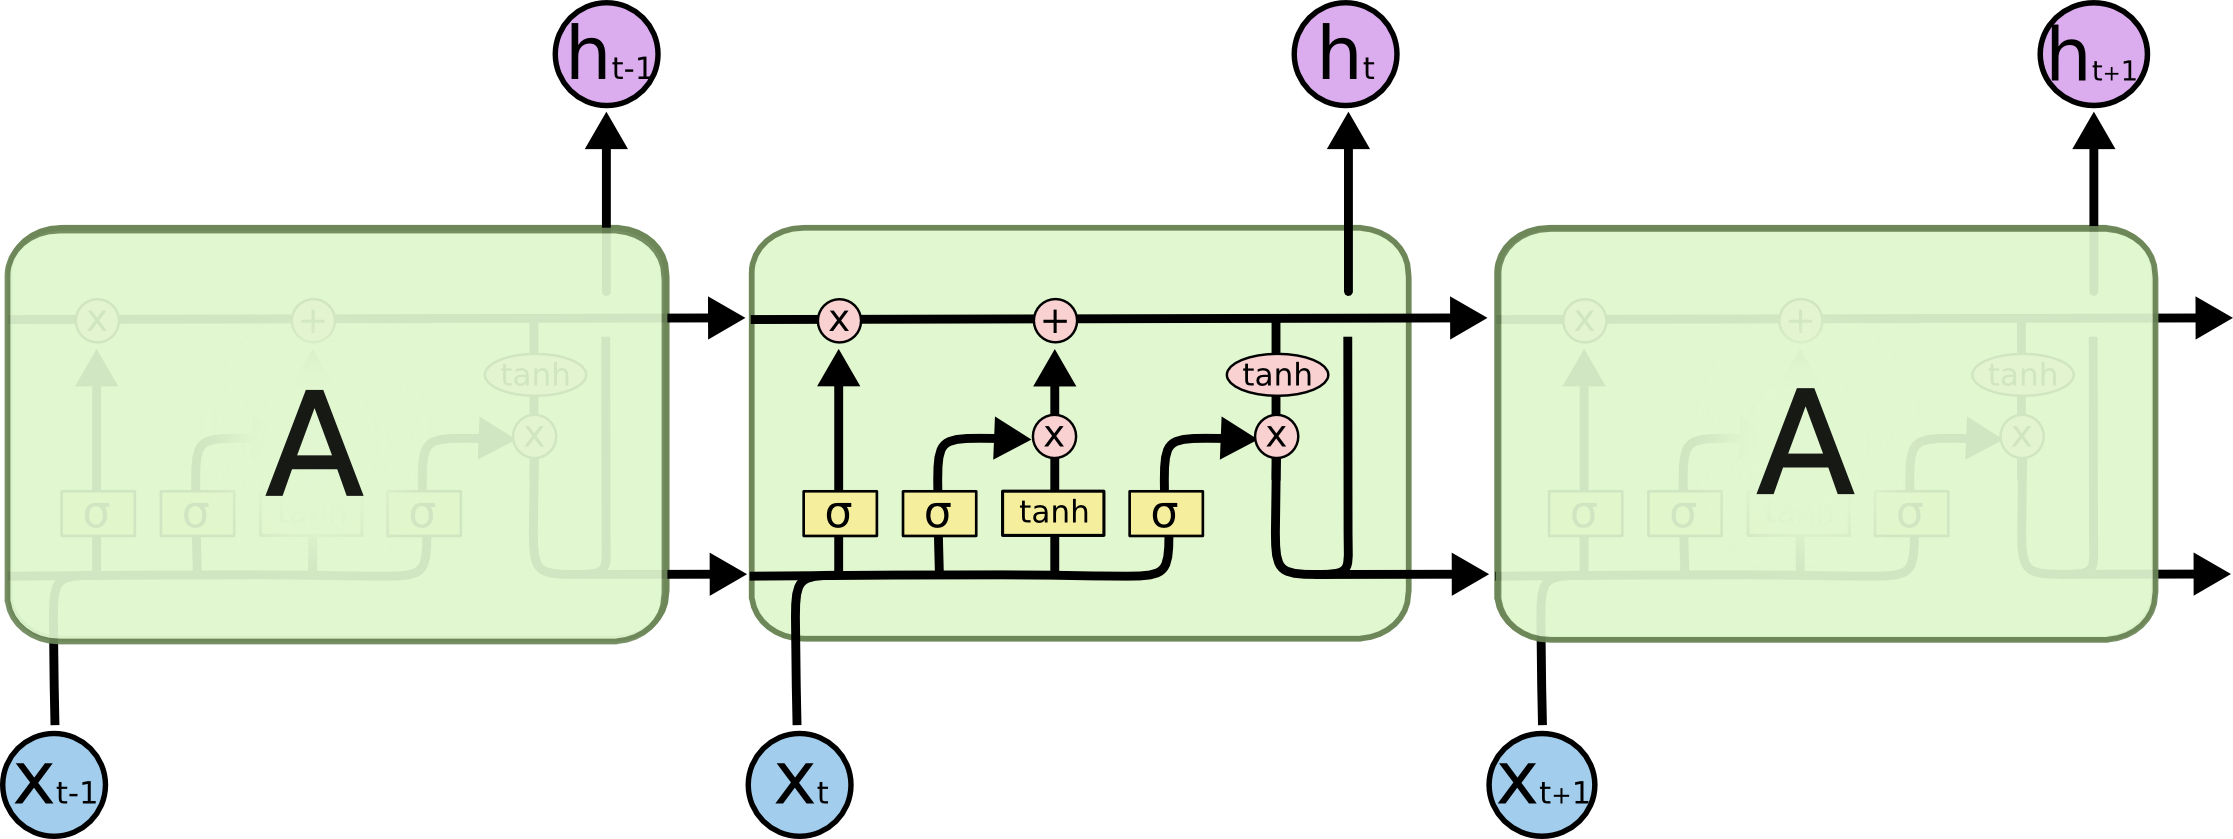
\includegraphics[width=0.9\textwidth]{pics/LSTMchain.png} % Ajustado el ancho
        \caption{Diagrama general de una cadena LSTM.}
    \end{figure}
    \begin{block}{Flujo de información}
        La imagen muestra cómo la información ($\vect{x}_t$), el estado oculto ($\vect{h}_{t-1}$) y el estado de celda ($\vect{c}_{t-1}$) fluyen a través de las compuertas para generar las nuevas versiones ($\vect{h}_t$, $\vect{c}_t$).
    \end{block}
\end{frame}

\begin{frame}
    \frametitle{LSTM: compuerta de olvido}
    \begin{block}{1. Compuerta de olvido ($\vect{f}_t$)}
        Decide qué información desechar del estado de celda anterior $\vect{c}_{t-1}$. Basada en $\vect{h}_{t-1}$ y $\vect{x}_t$.
        \[ \vect{f}_t = \sigma(\mat{W}_f [\vect{h}_{t-1}, \vect{x}_t] + \vect{b}_f) \]
        ($\sigma$: sigmoide. $\vect{f}_t \in [0, 1]$. $1$=mantener, $0$=olvidar)
    \end{block}
\end{frame}

\begin{frame}
    \frametitle{LSTM: Compuerta de entrada}
    \begin{block}{2. Compuerta de entrada ($\vect{i}_t$, $\tilde{\vect{c}}_t$)}
        Decide qué nueva información almacenar en $\vect{c}_t$.
        \begin{itemize}
            \item \textit{Qué valores actualizar} ($\vect{i}_t \in [0, 1]$):
            \[ \vect{i}_t = \sigma(\mat{W}_i [\vect{h}_{t-1}, \vect{x}_t] + \vect{b}_i) \]
            \item \textit{Valores candidatos a añadir} ($\tilde{\vect{c}}_t \in [-1, 1]$):
            \[ \tilde{\vect{c}}_t = \tanh(\mat{W}_c [\vect{h}_{t-1}, \vect{x}_t] + \vect{b}_c) \]
        \end{itemize}
        Luego, actualiza estado de celda: $\vect{c}_t = \vect{f}_t * \vect{c}_{t-1} + \vect{i}_t * \tilde{\vect{c}}_t$ (\textbf{Adición!})
    \end{block}
\end{frame}

\begin{frame}
    \frametitle{LSTM: Compuerta de salida y estado oculto}
    \begin{block}{3. Compuerta de salida ($\vect{o}_t$)}
         Decide qué partes del estado de celda $\vect{c}_t$ exponer.
         \[ \vect{o}_t = \sigma(\mat{W}_o [\vect{h}_{t-1}, \vect{x}_t] + \vect{b}_o) \]
    \end{block}
    \begin{block}{Estado oculto ($\vect{h}_t$)}
         Calcula el estado oculto (salida de la celda).
         \[ \vect{h}_t = \vect{o}_t * \tanh(\vect{c}_t) \]
         ($*$: multiplicación elemento a elemento)
    \end{block}
\end{frame}

\begin{frame}
    \frametitle{LSTM: ¿cómo resuelve el vanishing gradient?}
    \begin{block}{El rol clave del estado de celda ($\vect{c}_t$)}
        % \[ \vect{c}_t = \underbrace{\vect{f}_t * \vect{c}_{t-1}}_{\text{Olvidar/Mantener}} \quad + \quad \underbrace{\vect{i}_t * \tilde{\vect{c}}_t}_{\text{Añadir nuevo}} \]
        \begin{itemize}
            \item La operación \textbf{aditiva} ($\vect{c}_t = \dots + \dots$) es crucial. Permite que la información (y gradientes) fluyan más fácilmente.
            \item Si $f_t \approx 1$ y $i_t \approx 0$, entonces $\vect{c}_t \approx \vect{c}_{t-1}$. La información se preserva casi intacta $\rightarrow$ ``autopista'' para el gradiente.
            \item Evita la multiplicación repetida de términos pequeños que causa el desvanecimiento en RNN simples.
            \item Las compuertas \textbf{aprenden} cuándo preservar y cuándo actualizar la memoria.
        \end{itemize}
    \end{block}
\end{frame}


% -------------------------------------------------------------------
\subsection{GRU (Gated Recurrent Unit)}
% -------------------------------------------------------------------

\begin{frame}
    \frametitle{GRU: una alternativa simplificada}
        \begin{block}{Concepto (Cho et al., 2014)}
            \begin{itemize}
                \item Simplifica la arquitectura LSTM.
                \item Combina estado de celda y oculto en $\vect{h}_t$.
                \item Solo \textbf{dos compuertas}:
                    \begin{itemize}
                        \item Actualización ($\vect{z}_t$).
                        \item Reinicio ($\vect{r}_t$).
                    \end{itemize}
                \item Menos parámetros, más eficiente.
            \end{itemize}
        \end{block}
\end{frame}

\begin{frame}
    \frametitle{GRU: diagrama de la celda}
    \begin{figure}
        \centering
        \includegraphics[width=0.7\textwidth]{pics/gru_diagram.png} % Ajustado el ancho
        \caption{Diagrama detallado de una celda GRU.}
    \end{figure}
    % \begin{block}{Flujo de información en GRU}
    %     \begin{itemize}
    %         \item La celda recibe la entrada $\vect{x}_t$ y el estado anterior $\vect{h}_{t-1}$.
    %         \item La \textbf{compuerta de reinicio ($\vect{r}_t$)} decide cuánto olvidar de $\vect{h}_{t-1}$ para calcular el estado candidato $\tilde{\vect{h}}_t$.
    %         \item La \textbf{compuerta de actualización ($\vect{z}_t$)} controla la mezcla entre el estado anterior $\vect{h}_{t-1}$ y el candidato $\tilde{\vect{h}}_t$ para formar el nuevo estado $\vect{h}_t$.
    %     \end{itemize}
    % \end{block}
\end{frame}

\begin{frame}
    \frametitle{GRU: Compuerta de reinicio}
    %  \begin{figure}
    %     \centering
    %     % \includegraphics[width=0.8\textwidth]{pics/gru_reset_gate.png}
    %     \vspace{0.5cm}
    %     (Diagrama GRU: Foco en Reinicio)
    % \end{figure}
    \begin{block}{1. Compuerta de reinicio ($\vect{r}_t$)}
        Decide cuánto del estado anterior $\vect{h}_{t-1}$ ``olvidar'' al calcular la info candidata $\tilde{\vect{h}}_t$.
        \[ \vect{r}_t = \sigma(\mat{W}_r [\vect{h}_{t-1}, \vect{x}_t] + \vect{b}_r) \]
        Calcula el estado candidato $\tilde{\vect{h}}_t$:
        \[ \tilde{\vect{h}}_t = \tanh(\mat{W}_h [\vect{r}_t * \vect{h}_{t-1}, \vect{x}_t] + \vect{b}_h) \]
         ($\vect{r}_t \approx 0 \implies$ ignora $\vect{h}_{t-1}$ para el candidato).
    \end{block}
\end{frame}

\begin{frame}
    \frametitle{GRU: compuerta de actualización y estado final}
     \begin{block}{2. Compuerta de actualización ($\vect{z}_t$)}
        Decide cuánto mantener de $\vect{h}_{t-1}$ vs. cuánto incorporar de $\tilde{\vect{h}}_t$.
         \[ \vect{z}_t = \sigma(\mat{W}_z [\vect{h}_{t-1}, \vect{x}_t] + \vect{b}_z) \]
    \end{block}
     \begin{block}{Estado final ($\vect{h}_t$)}
         Calcula el estado final (interpolación):
         \[ \vect{h}_t = (1 - \vect{z}_t) * \vect{h}_{t-1} + \vect{z}_t * \tilde{\vect{h}}_t \]
    \end{block}
    \begin{center} \footnotesize \bigskip
    \textit{Estructura aditiva ayuda a mitigar vanishing gradient.}
    \end{center}
\end{frame}

\section{Cierre y reflexión}
\begin{frame}
    \frametitle{¿Cuándo elegir cada modelo?}
    \begin{block}{Guía general}
        \begin{itemize}
            \item \textbf{RNN Simple (Elman):}
                \begin{itemize}
                    \item \textit{Cuándo:} Rara vez hoy día. Quizás para secuencias muy cortas, problemas muy simples, fines educativos.
                    \item \textit{Por qué:} Sufre mucho con dependencias largas (vanishing gradient).
                \end{itemize} \bigskip
            \item \textbf{LSTM:}
                 \begin{itemize}
                    \item \textit{Cuándo:} Tareas con dependencias potencialmente muy largas, robustez clave, recursos computacionales suficientes. Era el ``caballo de batalla''.
                    \item \textit{Por qué:} Buen manejo de memoria larga, arquitectura probada.
                \end{itemize}
        \end{itemize}
    \end{block}
\end{frame}

\begin{frame}
    \frametitle{¿Cuándo elegir cada modelo?}
    \begin{block}{Guía general}
        \begin{itemize}
            \item \textbf{GRU:}
                 \begin{itemize}
                    \item \textit{Cuándo:} Similar a LSTM, pero se busca mayor eficiencia (rapidez, menos parámetros), o datos limitados. Buena primera opción a probar.
                    \item \textit{Por qué:} Equilibrio rendimiento/eficiencia.
                \end{itemize} \bigskip
                \item \textbf{BiRNN (BiLSTM/BiGRU):}
                \begin{itemize}
                   \item \textit{Cuándo:} Tareas \textit{offline} (secuencia completa disponible) donde contexto futuro ayuda (etiquetado, codificación seq2seq).
                \end{itemize} \bigskip
            \end{itemize}
    \end{block}
\end{frame}

\begin{frame}
    \frametitle{¿Cuándo elegir cada modelo?}
    \begin{block}{Guía general}
        \begin{itemize}
             \item \textbf{Stacked RNN (Stacked LSTM/GRU):}
                  \begin{itemize}
                    \item \textit{Cuándo:} Modelar jerarquías complejas, si más profundidad mejora rendimiento (con suficiente data/regularización).
                  \end{itemize}
        \end{itemize}
         \bigskip \textit{Nota: Los Transformers ahora dominan muchas de estas tareas.}
    \end{block}
\end{frame}

\begin{frame}
    \frametitle{El panorama actual y futuro: Transformers}
    \begin{block}{La era de los Transformers}
        \begin{itemize}
            \item Arquitecturas basadas en \textbf{mecanismos de atención} (ej. Transformer) han superado a las RNNs en muchas tareas SOTA de NLP desde ~2017 (Attention is All You Need).
            \item \textbf{Ventajas clave de Transformers:}
                \begin{itemize}
                    \item Mejor manejo de dependencias muy largas (acceso directo, no secuencial).
                    \item Mayor paralelización (entrenamiento más rápido en hardware adecuado).
                \end{itemize}
        \end{itemize}
    \end{block}
\end{frame}

\begin{frame}
    \frametitle{¿Están obsoletas las RNNs?}
    \begin{block}{¡No! Siguen siendo relevantes}
                \begin{itemize}
                    \item \textbf{Procesamiento online/streaming:} Donde la secuencia llega paso a paso y el futuro no se conoce.
                    \item \textbf{Eficiencia:} Pueden ser más ligeras (menos parámetros/cómputo) que Transformers grandes, útil en recursos limitados.
                    \item \textbf{Tareas específicas:} Donde la naturaleza secuencial inherente es ventajosa o suficiente.
                    \item \textbf{Bloques constructivos:} Usadas en arquitecturas híbridas.
                    \item \textbf{Fundamento conceptual:} Comprender RNNs/LSTM/GRU es clave para entender la evolución del campo.
                \end{itemize}
    \end{block}
\end{frame}

\begin{frame}
    \frametitle{Resumen y conclusiones}
    \begin{block}{Puntos clave}
        \begin{itemize}
            \item El NLP requiere modelos que manejen \textbf{secuencias} y \textbf{memoria}.
            \item Las \textbf{RNNs} introducen recurrencia ($\vect{h}_t$ depende de $\vect{h}_{t-1}$), pero las simples sufren de \textbf{problemas de gradiente} (vanishing/exploding).
        \end{itemize}
    \end{block}
\end{frame}

\begin{frame}
    \frametitle{Resumen y conclusiones}
    \begin{block}{Puntos clave}
        \begin{itemize}
            \item \textbf{BiRNNs} usan contexto pasado y futuro; \textbf{Stacked RNNs} aumentan la profundidad.
            \item \textbf{LSTM} y \textbf{GRU} introducen \textbf{compuertas} para controlar flujo de información/gradientes, modelando eficazmente dependencias largas.
            \item La elección del modelo (RNN simple, LSTM, GRU, Bi, Stacked) depende de la tarea, datos, dependencias y recursos.
        \end{itemize}
    \end{block}
\end{frame}

\begin{frame}
    \frametitle{Resumen y conclusiones}
    \begin{block}{Puntos clave}
        \begin{itemize}
            \item Aunque los \textbf{Transformers} dominan actualmente muchas tareas SOTA, las RNNs siguen siendo relevantes y conceptualmente fundacionales.
        \end{itemize}
    \end{block}
\end{frame}

% -------------------------------------------------------------------
% REFERENCIAS
% -------------------------------------------------------------------
\begin{frame}[allowframebreaks]
 \frametitle{Referencias}
 \bibliographystyle{apalike}
 \begin{thebibliography}{9}
     \bibitem{Hochreiter1997} Hochreiter, S., \& Schmidhuber, J. (1997). Long short-term memory. \textit{Neural computation}, 9(8), 1735-1780.
     \bibitem{Cho2014} Cho, K., et al. (2014). Learning phrase representations using RNN encoder-decoder for statistical machine translation. \textit{arXiv:1406.1078}.
     \bibitem{Elman1990} Elman, J. L. (1990). Finding structure in time. \textit{Cognitive science}, 14(2), 179-211.
     \bibitem{Vaswani2017} Vaswani, A., et al. (2017). Attention is all you need. \textit{NIPS}.
\end{thebibliography}
\end{frame}
% -------------------------------------------------------------------

\end{document}
